\chapter{Appendix 2: Analysis of the network embedding learned from local, global structural and time components}
\label{appendix:k-means_time_struc}

\begin{figure}[!ht]
	\centering
	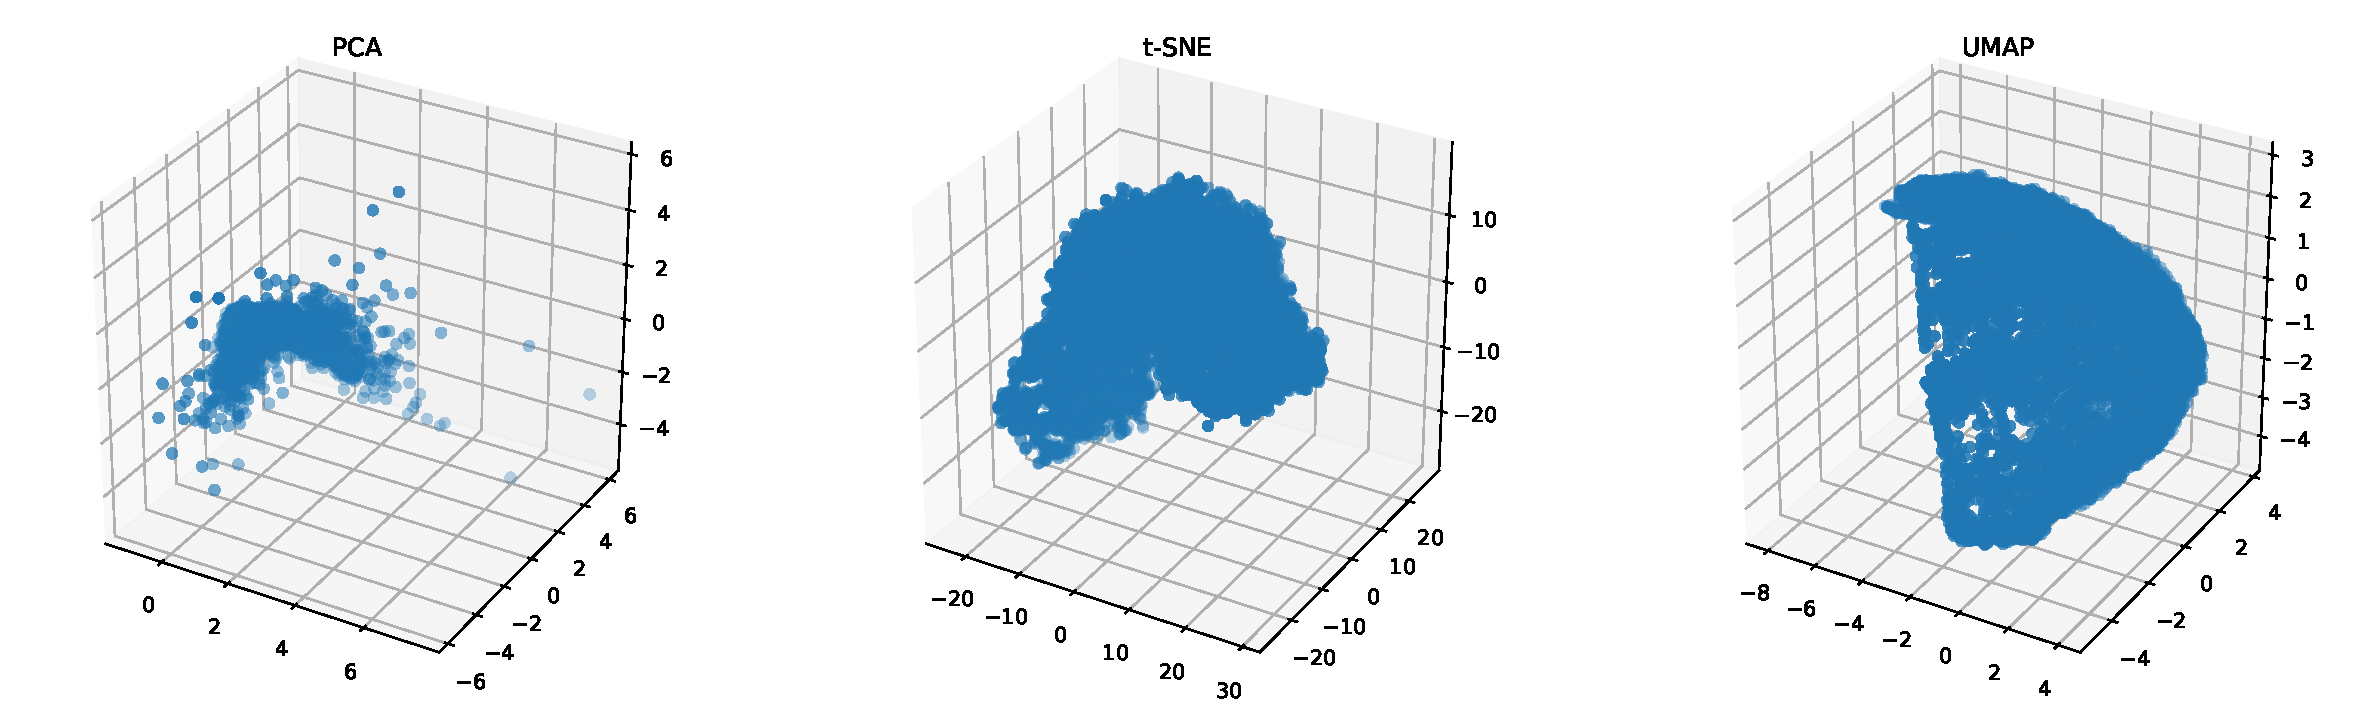
\includegraphics[width=1.0\textwidth]{images/appendix/App5.pdf}\\
	\caption{Embedding set reduced to 3 dimensions by three dimensionality reduction techniques.}
	\label{fig:App5}
\end{figure}
\begin{figure}[!ht]
	\centering
	\includegraphics[width=1.0\textwidth]{images/appendix/App6.pdf}\\
	\caption{Elbow plots for 3-dimensional embedding sets.}
	\label{fig:App6}
\end{figure}
\begin{figure}[!ht]
	\centering
	\includegraphics[width=1.0\textwidth]{images/appendix/App7.pdf}\\
	\caption{Evaluation of $k$-means clustering with respect to the number of clusters $k$.}
	\label{fig:App7}
\end{figure}
\begin{figure}[!ht]
	\centering
	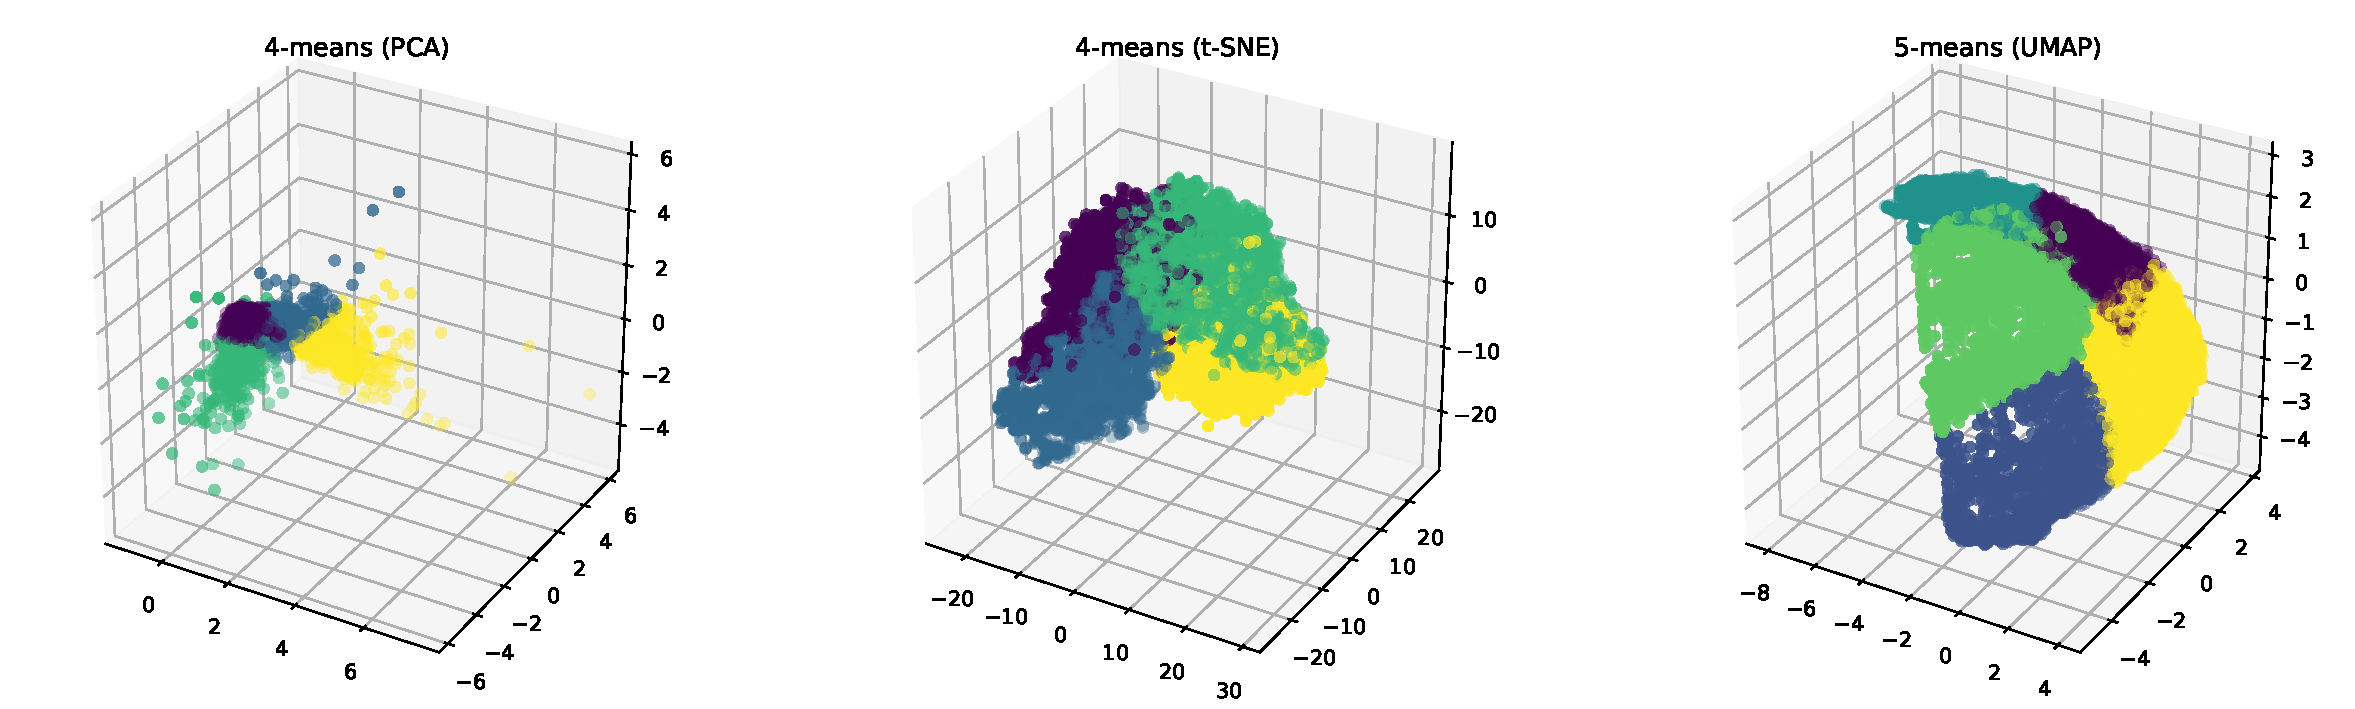
\includegraphics[width=1.0\textwidth]{images/appendix/App8.pdf}\\
	\caption{Resulting $k$-means clustering.}
	\label{fig:App8}
\end{figure}

\begin{figure}[!ht]
	\centering
	\includegraphics[width=1.0\textwidth]{images/appendix/App11.pdf}\\
	\caption{Evaluation of HDBSCAN clustering with respect to the set of hyperparameters.}
	\label{fig:App11}
\end{figure}
\begin{figure}[!ht]
	\centering
	\includegraphics[width=1.0\textwidth]{images/appendix/App12.pdf}\\
	\caption{Resulting HDBSCAN clustering.}
	\label{fig:App12}
\end{figure}

